\documentclass[twoside]{article}

% Packages required by doxygen
\usepackage{fixltx2e}
\usepackage{calc}
\usepackage{doxygen}
\usepackage[export]{adjustbox} % also loads graphicx
\usepackage{graphicx}
\usepackage[utf8]{inputenc}
\usepackage{makeidx}
\usepackage{multicol}
\usepackage{multirow}
\PassOptionsToPackage{warn}{textcomp}
\usepackage{textcomp}
\usepackage[nointegrals]{wasysym}
\usepackage[table]{xcolor}

% NLS support packages
\usepackage[french]{babel}

% Font selection
\usepackage[T1]{fontenc}
\usepackage[scaled=.90]{helvet}
\usepackage{courier}
\usepackage{amssymb}
\usepackage{sectsty}
\renewcommand{\familydefault}{\sfdefault}
\allsectionsfont{%
  \fontseries{bc}\selectfont%
  \color{darkgray}%
}
\renewcommand{\DoxyLabelFont}{%
  \fontseries{bc}\selectfont%
  \color{darkgray}%
}
\newcommand{\+}{\discretionary{\mbox{\scriptsize$\hookleftarrow$}}{}{}}

% Page & text layout
\usepackage{geometry}
\geometry{%
  a4paper,%
  top=2.5cm,%
  bottom=2.5cm,%
  left=2.5cm,%
  right=2.5cm%
}
\tolerance=750
\hfuzz=15pt
\hbadness=750
\setlength{\emergencystretch}{15pt}
\setlength{\parindent}{0cm}
\setlength{\parskip}{3ex plus 2ex minus 2ex}
\makeatletter
\renewcommand{\paragraph}{%
  \@startsection{paragraph}{4}{0ex}{-1.0ex}{1.0ex}{%
    \normalfont\normalsize\bfseries\SS@parafont%
  }%
}
\renewcommand{\subparagraph}{%
  \@startsection{subparagraph}{5}{0ex}{-1.0ex}{1.0ex}{%
    \normalfont\normalsize\bfseries\SS@subparafont%
  }%
}
\makeatother

% Headers & footers
\usepackage{fancyhdr}
\pagestyle{fancyplain}
\fancyhead[LE]{\fancyplain{}{\bfseries\thepage}}
\fancyhead[CE]{\fancyplain{}{}}
\fancyhead[RE]{\fancyplain{}{\bfseries\leftmark}}
\fancyhead[LO]{\fancyplain{}{\bfseries\rightmark}}
\fancyhead[CO]{\fancyplain{}{}}
\fancyhead[RO]{\fancyplain{}{\bfseries\thepage}}
\fancyfoot[LE]{\fancyplain{}{}}
\fancyfoot[CE]{\fancyplain{}{}}
\fancyfoot[RE]{\fancyplain{}{\bfseries\scriptsize Généré le \today ~pour Destinie2 par Doxygen }}
\fancyfoot[LO]{\fancyplain{}{\bfseries\scriptsize Généré le \today ~pour Destinie2 par Doxygen }}
\fancyfoot[CO]{\fancyplain{}{}}
\fancyfoot[RO]{\fancyplain{}{}}
\renewcommand{\footrulewidth}{0.4pt}
\renewcommand{\sectionmark}[1]{%
  \markright{\thesection\ #1}%
}

% Indices & bibliography
\usepackage{natbib}
\usepackage[titles]{tocloft}
\setcounter{tocdepth}{3}
\setcounter{secnumdepth}{5}
\makeindex

% Packages requested by user
\usepackage{booktabs}
\usepackage{lscape}
\usepackage{natbib}
\usepackage{listings}
\usepackage{color}

\definecolor{dkgreen}{rgb}{0,0.6,0}
\definecolor{gray}{rgb}{0.5,0.5,0.5}
\definecolor{mauve}{rgb}{0.58,0,0.82}

\lstset{frame=tb,
language=R,
aboveskip=3mm,
belowskip=3mm,
showstringspaces=false,
columns=flexible,
numbers=none,
keywordstyle=\color{blue},
numberstyle=\tiny\color{gray},
commentstyle=\color{dkgreen},
stringstyle=\color{mauve},
breaklines=true,
breakatwhitespace=true,
tabsize=3
}
% Hyperlinks (required, but should be loaded last)
\usepackage{ifpdf}
\ifpdf
  \usepackage[pdftex,pagebackref=true]{hyperref}
\else
  \usepackage[ps2pdf,pagebackref=true]{hyperref}
\fi
\hypersetup{%
  colorlinks=true,%
  linkcolor=blue,%
  citecolor=blue,%
  unicode%
}

% Custom commands
\newcommand{\clearemptydoublepage}{%
  \newpage{\pagestyle{empty}\cleardoublepage}%
}

\usepackage{caption}
\captionsetup{labelsep=space,justification=centering,font={bf},singlelinecheck=off,skip=4pt,position=top}

%===== C O N T E N T S =====

\begin{document}

% Titlepage & ToC
\hypersetup{pageanchor=false,
             bookmarksnumbered=true,
             pdfencoding=unicode
            }
\pagenumbering{alph}
\begin{titlepage}
\vspace*{7cm}
\begin{center}%
{\Large Destinie2 }\\
\vspace*{1cm}
{\large Généré par Doxygen 1.8.12}\\
\vspace*{0.5cm}
{\small \today }\\
\end{center}
\end{titlepage}
\pagenumbering{roman}
\tableofcontents
\pagenumbering{arabic}
\hypersetup{pageanchor=true}

%--- Begin generated contents ---

\section{Introduction}
Destinie 2 est un modèle de microsimulation dynamique, développé à l'Insee, qui permet de projeter les retraites aux niveaux individuel et agrégé à long terme. Il repose sur un échantillon représentatif de la population française au 1er janvier 2010, construit à partir de l'enquête Patrimoine 2009-2010 et composé de 62 000 individus. Ce modèle projette les situations familiales, carrières professionnelles et départs à la retraite des personnes de cette population, dont le renouvellement est assuré par la simulation des naissances, décès et flux migratoires. Les individus sont répartis en trois grands groupes : les salariés du secteur privé, les titulaires de la fonction publique et les indépendants. Au niveau d’un individu, Destinie 2 permet de suivre l’ensemble de sa trajectoire professionnelle (statuts d’activité et revenus), et simule les liquidations à la retraite sous diverses hypothèses de comportement et de législation. Les liens familiaux (unions, naissances, séparations) étant simulés, ce modèle permet également de réaliser des estimations au niveau du ménage.\\
Le modèle comprend deux modules distincts : le module générateur de biographies et le module de simulation des droits retraite.
La constitution des biographies démographiques s'appuie sur les dernières projections démographiques de l'Insee, couvrant la période 2013-2070 et le champ France entière. Les trajectoires professionnelles des individus sont connues jusqu’en 2009, année de base. \`A compter de 2010, leurs carrières (statuts d’activité et revenus) sont projetées en respectant des contraintes de calage sur des hypothèses macroéconomiques. Ces hypothèses portent sur la croissance de la productivité du travail et le taux de chômage, fournis par le COR, et le taux d'activité, repris des projections de population active de l'Insee.
Le module retraite simule le départ à la retraite selon la date de législation et l'hypothèse de comportement de liquidation choisies, et calcule le montant des droits associés. Les droits couvrent la pension de droit direct et de réversion des régimes de base (régime général, SRE et CNRACL, RSI) et complémentaires (Arrco, Agirc). La dimension ménage permet d'inclure le minimum vieillesse.\\
Ce document détaille le contenu des fichiers de code source du modèle. 



\section{Vue d'ensemble}

Le programme est un package R écrit en C++. Il peut
être directement utilisé à partir d'une console en R, 
pour effectuer des simulations en fonction d'un échantillon
directement importable en R, et en passant les paramètres de la simulation
toujours depuis R. En revanche, le package en lui-même est écrit en C++. 

Structure des répertoires du package :


	\begin{description}
		\item[src] contient les fichiers sources écrits en C++ du package
		\item[R] contient les fichiers sources écrits en R du package
		\item[parametres] contient les paramètres démographiques et macroéconomiques utilisés lors de la projection\\
Le sous-répertoire {\tt Projections\_COR\_2018} comprend les 5 scénarios économiques du rapport de juin 2018 du COR. 
\renewcommand{\arraystretch}{1.8}
\newcolumntype{C}{>{\centering\arraybackslash}X}

\begin{table}[h]
  \centering
  \caption{Scénarios économiques du COR}
    \begin{tabular}{rr}
    \toprule
 Croissance du SMPT & Taux de chômage \\
    \midrule
 1,8     & 4,5 \\
 1,8   & 7 \\
 1,5   & 7 \\
 1,3   & 7 \\
 1     & 7 \\
 1     & 10 \\
    \bottomrule
    \end{tabular}%
  \label{tab:hypscCOR}%
\end{table}%
		\item[test] contient un échantillon test \textbf{non représentatif} de la population mais que l'on peut utiliser pour prendre en main le modèle de microsimulation
		\item[documentation] contient la documentation du package, la liste des documents de travail de l'Insee publiés à partir du modèle Destinie 2 et la liste des contributeurs du modèle.
	\end{description}






\subsection{Le package Destinie}


Le programme est structuré principalement autour de cinq classes d'objets et de structures.
La classe Simulation contient l'ensemble des paramètres d'une simulation ainsi que 
l'échantillon issu du générateur de biographies
utilisé sous la forme d'un tableau d'objets Indiv.
La classe Indiv contient l'ensemble de l'information d'un individu donné.
La classe Retraite contient les variables sur les pensions (de droit direct ou dérivé) 
pour un individu et une année donnée.
La classe DroitsRetr contient l'ensemble des variables concernant la liquidation des
droits directs.
La classe Legislation contient l'ensemble des paramètres législatifs pour une 
date de législation, une année et un individu donné. 
La structure Macro contient l'ensemble des paramètres macroéconomiques (PIB, inflation,...) mais aussi des 
paramètres plus spécifiques aux retraites (taux de cotisation, valeur des points dans les complémentaires ou encore montant du minimum vieillesse).

Outre ces cinq classes, 
les fichiers {\tt Demographie.cpp}  et {\tt Destinie.h} contiennent les fonctions qui peuvent être appelées directement depuis R,
ainsi que les constantes du modèles.
Le fichier {\tt OutilsBase.h}, quant à lui, contient des fonctions utilitaires.



\phantom{sdfgsdgf
sdfgsdg}

\medskip 

\begin{landscape}
\begin{figure}
\caption{Structure générale du package}
\label{fig:structGenePack}
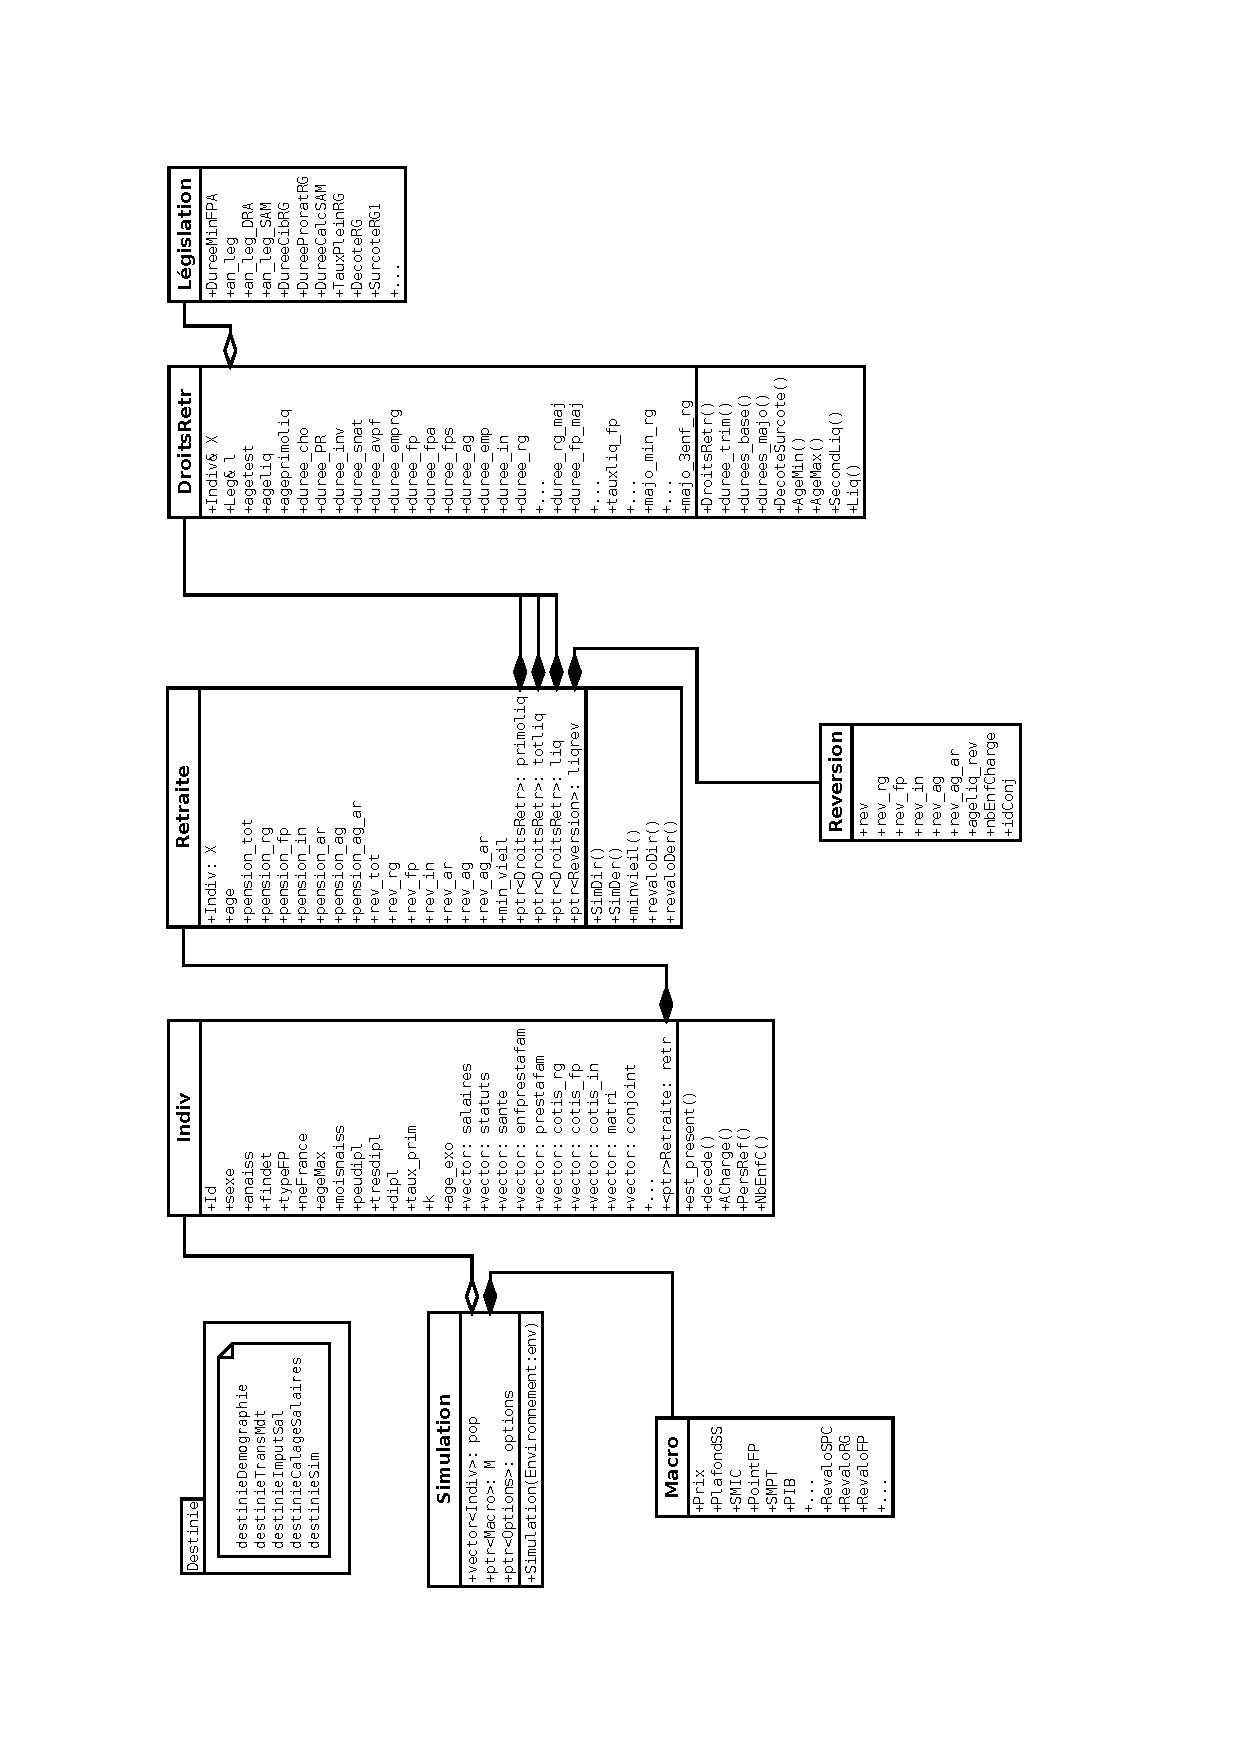
\includegraphics[scale=0.85,angle=270,origin=c]{Diagramme2.pdf}
\end{figure}
\end{landscape}


\subsection{Choix de Législation possibles}

\subsubsection{Réforme de 1993}

\begin{itemize}
\item	Concerne uniquement les salariés du secteur privé et les régimes alignés ;
\item Allongement progressif de la durée d'assurance requise pour accéder au taux plein (modification progressive pour les générations 1934-1943 à raison d'un trimestre supplémentaire par génération) ;
\item	Calcul du salaire de référence sur les 25 meilleures années au lieu de 10 (modification progressive pour les générations 1934-1947 à raison d'une année supplémentaire par génération) ;
\item	Les pensions et les salaires portés au compte sont indexés sur les prix, et non plus sur les salaires (principe déjà en vigueur depuis 1987) ;
\end{itemize}
\href{http://www.legislation.cnav.fr/textes/cr/cn/TLR-CR_CN_10393_30121993.htm#323}%
{Circulaire n°103/93 du 30 décembre 1993 Caisse nationale d'assurance vieillesse}
% Table generated by Excel2LaTeX from sheet 'Feuil2'
\begin{table}[h]
  \centering
  \caption{Détail par génération de la période transitoire 1993}
    \begin{tabular}{rrr}
    \toprule
    Année de  & Nombre d'années retenues & Trimestres d'assurance  \\
    naissance & pour le calcul du SAM    & pour obtenir le taux plein \\
    \midrule
    1933 et avant & 10    & 150 \\
    1934  & 11    & 151 \\
    1935  & 12    & 152 \\
    1936  & 13    & 153 \\
    1937  & 14    & 154 \\
    1938  & 15    & 155 \\
    1939  & 16    & 156 \\
    1940  & 17    & 157 \\
    1941  & 18    & 158 \\
    1942  & 19    & 159 \\
    1943  & 20    & 160 \\
    1944  & 21    & 160 \\
    1945  & 22    & 160 \\
    1946  & 23    & 160 \\
    1947  & 24    & 160 \\
    1948 et au-delà & 25    & 160 \\
    \bottomrule
    \end{tabular}%
  \label{tab:addlabel}%
\end{table}%


\subsubsection{Réforme de 2003}

\paragraph{Le régime général}

\begin{itemize}
   \item	Allongement progressif de la durée d'assurance requise pour accéder au taux plein à partir de la génération 1949 (passage de 160 
         trimestres à 164)
   \item	Allongement de la durée intervenant dans le coefficient de proratisation, censée à terme évoluer comme la durée cible d'assurance
   \item	Réduction de la décote à partir de la génération 1944, de 0,5 point par an pour atteindre 5\% par annuité manquante pour les 
         générations nées après 1952 (la décôte n'est appliquée que si la liquidation a lieu avant 65 ans)
   \item	Surcote de 3\% par année supplémentaire travaillée après le 1er janvier 2004 ; la surcote a été renforcée par le plan « emploi des 
seniors » au printemps 2005
   \item	Modification du mode de calcul du minimum contributif
   \item	Possibilité de départ anticipé pour carrière longue : depuis le 1er janvier 2004, les assurés qui ont commencé à travailler très 
         jeune (avant 18 ans), et qui ont eu une longue carrière  peuvent partir à la retraite avant 60 ans (la condition de début de carrière est 
         un obstacle pour les assurés nés à partir de 1953 qui ont connu une scolarité obligatoire jusqu'à 16 ans).
\end{itemize}

% Table generated by Excel2LaTeX from sheet 'Feuil2'
\begin{table}[h]
  \centering
  \caption{Détail par génération de la période transitoire 2003}
    \begin{tabular}{rrrrr}
    \toprule
              &                   & Trimestres    &                       & Trimestres \\
              & Nombre d'années   & d'assurance   & Minoration du taux    & d'assurance   \\
    Année de  & retenues pour     & pour obtenir  & par nombre de         & maximum retenus        \\
    naissance & le calcul du SAM  & le taux plein & trimestre manquant    & pour le calcul RG      \\
    \midrule
    1933 et avant & 10    & 150   & \multicolumn{1}{r}{\multirow{11}[0]{*}{-1,2500}} & \multicolumn{1}{r}{\multirow{11}[0]{*}{150}} \\
    1934  & 11    & 151   & \multicolumn{1}{c}{} & \multicolumn{1}{c}{} \\
    1935  & 12    & 152   & \multicolumn{1}{c}{} & \multicolumn{1}{c}{} \\
    1936  & 13    & 153   & \multicolumn{1}{c}{} & \multicolumn{1}{c}{} \\
    1937  & 14    & 154   & \multicolumn{1}{c}{} & \multicolumn{1}{c}{} \\
    1938  & 15    & 155   & \multicolumn{1}{c}{} & \multicolumn{1}{c}{} \\
    1939  & 16    & 156   & \multicolumn{1}{c}{} & \multicolumn{1}{c}{} \\
    1940  & 17    & 157   & \multicolumn{1}{c}{} & \multicolumn{1}{c}{} \\
    1941  & 18    & 158   & \multicolumn{1}{c}{} & \multicolumn{1}{c}{} \\
    1942  & 19    & 159   & \multicolumn{1}{c}{} & \multicolumn{1}{c}{} \\
    1943  & 20    & \multicolumn{1}{r}{\multirow{6}[0]{*}{160}} & \multicolumn{1}{r}{} & \multicolumn{1}{c}{} \\
    1944  & 21    & \multicolumn{1}{c}{} & -1,1875 & 152 \\
    1945  & 22    & \multicolumn{1}{c}{} & -1,1250 & 154 \\
    1946  & 23    & \multicolumn{1}{c}{} & -1,0625 & 156 \\
    1947  & 24    & \multicolumn{1}{c}{} & -1,0000 & 158 \\
    1948  & \multicolumn{1}{r}{\multirow{5}[0]{*}{25}} & \multicolumn{1}{r}{} & -0,9375 & 160 \\
    1949  & \multicolumn{1}{c}{} & 161   & -0,8750 & 161 \\
    1950  & \multicolumn{1}{c}{} & 162   & -0,8125 & 162 \\
    1951  & \multicolumn{1}{c}{} & 163   & -0,7500 & 163 \\
    1952  & \multicolumn{1}{c}{} & 164   & -0,6875 & 164 \\
    \bottomrule
    \end{tabular}%
  \label{tab:addlabel}%
\end{table}%

\paragraph{Fonction publique}

\begin{itemize}
	\item	Augmentation de la durée d'assurance à partir de 2004 pour rejoindre celle requise dans le régime général et ensuite progresser en 
         parallèle à partir de 2006
	\item	Décote de 0,5 point par annuité manquante, augmentée de 0,5 point à chaque génération pour atteindre 5\% en 2015 (avec hausse 
         progressive de l'âge pivot à partir duquel la décote s'annule)
	\item	Surcote de 3\% par année supplémentaire travaillée, comme dans le secteur privé
	\item	Modification du mode de calcul du minimum garanti
	\item	Modification des droits familiaux et conjugaux
\end{itemize}



\subsubsection{Réforme de 2010}

\begin{itemize}
	\item    le relèvement progressif de \textbf{l'âge légal de départ} à 
la retraite pour atteindre \textbf{62 ans} en 2018. Cette évolution 
concerne tous les salariés, du public comme du privé ainsi 
que les régimes spéciaux, mais avec des calendriers de mise 
en œuvre différents,
	\item    l'âge à partir duquel il est permis à un assuré, 
n'ayant pas la durée de cotisation requise, de bénéficier 
tout de même d'une retraite à taux plein, passe 
progressivement de \textbf{65 à 67 ans},
	\item    le dispositif des \textbf{"carrières longues"} est modifié, 
les salariés ayant commencé avant 18 ans peuvent partir à la 
retraite au plus tôt, sous réserve d'avoir la durée de 
cotisation requise pour leur génération, plus 2 ans.
	\item    pour les salariés qui, du fait d'une situation 
d'usure professionnelle, ont une incapacité physique 
supérieure ou égale à 20\%, l'âge légal de départ à la 
retraite reste fixé à 60 ans et aucune décote ne leur est 
appliquée,
	\item    les jeunes en chômage non indemnisé pourront 
valider jusqu'à 6 trimestres (au lieu de 4).
	% \item    pour les femmes, l'indemnité journalière perçue 
% pendant le congé maternité entrera dans le salaire de 
% référence sur lequel sera calculée la pension de retraite,
	% \item    de nouvelles recettes financières sont instaurées, 
% comme la hausse de la tranche la plus élevée de l'impôt sur 
% le revenu (\pct{41} au lieu de \pct{40}), l'augmentation des 
% taxes sur les stock-options et les retraites-chapeaux, le 
% relèvement des prélèvements forfaitaires sur les revenus du 
% capital et des taxes sur les dividendes perçus par les 
% actionnaires,
	% \item    l'objectif assigné au fonds de réserve des 
% retraites est modifié : ses réserves (36,2 milliards en 2010)
 % seront, à partir de 2011, ponctionnées annuellement (2,1 
% milliards) au profit de la Caisse d'amortissement de la 
% dette sociale (Cades). 
\end{itemize}

\subsubsection{Modification de la législation en 2011: accélération du calendrier fixé en 2010}

\subsubsection{Décret de juillet 2012: étendu du dispositif carrières longues}


\subsubsection{Réforme de 2013}
\begin{itemize}
   \item augmentation de la durée de cotisation d'un trimestre tous les 3 ans à partir de la génération née 
         en 1958 pour atteindre 43 ans pour la génération 1973.
   \item Périodes d'apprentissage, la formation, le chômage et la maternité mieux pris en compte
   \item Un trimestre est considéré comme validé dès que le salarié a cotisé 200 heures au smic. Désormais, ce seuil passera à 150 heures pour avantager les personnes à temps très partiel, avec un plafond fixé à 1,5 smic.
   \item Pour les salariés du public comme du privé, les cotisations patronales et salariales seront augmentées de 0,15 point chacune dès le 1er janvier 2014, puis de 0,05 point en 2015, 2016 et 2017. Le gouvernement a promis cependant de compenser la hausse du coût du travail pour les entreprises en 2014.
   \item Mise en place d'un compte pénibilité
   \item Le bonus pour les parents de trois enfants est fiscalisé
   \item La revalorisation des pensions décalée de six mois chaque année.
   \item Mise en place de la Lura (Liquidation unique des régimes alignés) à compter du 1er juillet 2017. Pour les individus ayant été affiliés à au moins deux des trois régimes affiliés (régime général, régime social des indépendants et MSA-salariés), et dont la liquidation intervient à partir du 1er juillet 2017, la pension est calculée de façon unifiée. Le salaire de référence est calculée sur la base des 25 meilleures années (tous régimes confondues), et la durée validée par année est bornée à quatre trimestres (par exemple, pour un individu ayant validé quatre trimestres au régime général et deux trimestres au RSI au cours d'une année, seuls quatre trimestres seront pris en compte dans la durée d'assurance). Le paiement de la pension due au titre des droits ouverts dans les trois régimes alignés est assuré par le dernier régime d’affiliation. Sur ce point, Destinie 2 s'écarte de la législation : la pension est en effet proratisée en fonction des durées validées dans chaque régime et les proratas sont comptés à la charge des régimes concernés.
\end{itemize}

\subsubsection{Accord national interprofessionnel relatif aux retraites complémentaires Agirc-Arrco du 30 octobre 2015}
\begin{itemize}
   \item en 2016, 2017 et 2018, indexation de la valeur du service des points Agirc et Arrco sur l'inflation moins un point
   \item en 2016, 2017 et 2018, indexation de la valeur d'achat des point Agirc et Arrco sur l'évolution du SMPT augmentée de deux points
   \item Extension de la cotisation AGFF sur la tranche B à la tranche C à compter du 1er janvier 2016
   \item Pour les individus liquidant leur retraite de base au taux plein, application d'un coefficient de minoration de 10\% sur la pension complémentaire, et ce, pour une durée de trois ans dans la limité de l'âge d'annulation de la décote. Ce coefficient ne s'applique pas aux individus qui liquident un an au moins après avoir rempli les conditions du taux plein. Pour les individus exonérés de la CSG ou soumis à un taux réduit, le coefficient ne s'applique pas ou est réduit
   \item Pour les individus remplissant les conditions du taux plein dans les régimes de base mais reportant leur liquidation de la retraite complémentaire d'au moins deux années, application, pour une durée d'un an, d'un coefficient majorant :
   \begin{itemize}
   \item de 10\% si la liquidation a lieu au moins deux ans après
   \item de 20\% si la liquidation a lieu au moins trois ans après
   \item de 30\% si la liquidation a lieu au moins quatre ans après
   \end{itemize}
\end{itemize}




\section{Index des classes}
\input{annotated}
\section{Index des fichiers}
\input{files}
\section{Documentation des classes}
\input{struct_cibles_demo}
\input{struct_cibles_trans}
%\input{struct_cibles_trans2}
\input{class_cotisations}
\input{struct_cotisations_t_r_i}
\input{struct_c_struct_sexe_age}
\input{class_droits_retr}
\input{struct_ech}
\input{struct_emp}
\input{struct_eq_salaires}
\input{struct_eq_sante}
\input{struct_eq_trans}
\input{struct_fam}
\input{struct_fin_etude_moy}
\input{struct_indic__annee}
\input{struct_indic__gen}
\input{struct_indic__gen__age}
\input{struct_indicateur}
\input{class_indiv}
\input{class_leg}
\input{struct_macro}
\input{struct_mortadiff__dip___f}
\input{struct_mortadiff__dip___h}
\input{struct_mortalite__diff}
%\input{struct_mortalite__diff__dip___f}
%\input{struct_mortalite__diff__dip___h}
\input{struct_moyenne}
\input{struct_opt}
\input{struct_option__optim}
\input{struct_options}
\input{struct_options__salaires}
\input{struct_options_t_r_i}
\input{structordre__findet}
\input{struct_paire}
\input{structquantile}
\input{struct_ratio}
\input{class_retraite}
\input{struct_retraite__comp}
\input{class_reversion}
\input{struct_salaire}
\input{struct_simulation}
\input{struct_somme}
\input{struct_taux}
\input{struct_transitions}
\section{Documentation des fichiers}
\input{_constantes_8h}
\input{_cotisations_8h}
\input{_cotisations_t_r_i_8h}
\input{_destinie_8h}
\input{_droits_retr_8h}
\input{_indicateurs__annee___c_o_r_8h}
\input{_indicateurs__gen_8h}
\input{_indicateurs__gen__age_8h}
\input{_indiv_8h}
\input{_legislation_8h}
\input{_migration_8h}
\input{_mortalite_8h}
\input{_naissance_8h}
\input{_outils_base_8h}
\input{_outils_comp_8h}
\input{_retraite_8h}
\input{_reversion_8h}
\input{_salaires_8h}
\input{_sante_8h}
\input{_separations_8h}
\input{_simulation_8h}
\input{_statistiques_8h}
\input{_transitions_8h}
\section{Guide de prise en main du modèle Destinie}
\subsection{Lancer une projection avec le modèle Destinie}
Ce guide vise à faciliter la première prise en main du modèle, tant pour des utilisateurs voulant utiliser le modèle dans sa forme actuelle (voir parties \ref{subsec::instmin} et \ref{subsec::simul}), que pour des utilisateurs plus experts voulant accéder au code source.\\
\subsubsection{Installation minimale}
\label{subsec::instmin}
\begin{enumerate}
\item Installations préalables : \\
\begin{itemize}
\item Installer	R (\url{https://cran.r-project.org/}) 
\item Installer	Rtools (\url{https://cran.r-project.org/bin/windows/Rtools/}), si votre système d'exploitation est 				Windows pour pouvoir installer le package destinie à partir des fichiers source. Choisir la version de Rtools compatible 		avec la version de R choisie précédemment. 
\end{itemize}
\item Installations recommandées : \\
\begin{itemize}
\item Installer	Rstudio (\url{https://www.rstudio.com/products/rstudio/download/}), environnement de travail R auquel il est parfois fait référence dans la documentation.
\item Installer git (\url{https://git-scm.com/}) de façon à pouvoir suivre les futures mises à jour du modèle.
\item Installer par exemple TortoiseGit (\url{https://tortoisegit.org/}) pour pouvoir utiliser Git en "clic-bouton".
\item Disposer d'un tableur (tel Microsoft Excel ou LibreOffice Calc).
\end{itemize}
\item Installer les packages nécessaires à Destinie :\\
\begin{lstlisting}
install.packages(c("devtools","pkgbuild"))
\end{lstlisting}
\item Installation du package Destinie :\\
L'installation se faisant à partir des fichiers sources, il est nécessaire pour les utilisateurs de Windows de lancer au préalable : 
\begin{lstlisting}
devtools::find_rtools()
# ou pkgbuild::find_rtools()
\end{lstlisting} pour obtenir un "TRUE".\\
Puis \begin{lstlisting}
devtools::install_github("InseeFr/Destinie-2",ref="release")
\end{lstlisting} (par défaut les packages dont dépend destinie seront installés)
\end{enumerate}

\subsubsection{Réaliser une première simulation}
\label{subsec::simul}
Dans le logiciel R,
\begin{enumerate}
\item On charge le package : \textit{library(destinie)}
\item On lance une simulation exemple : \textit{demo(simulation,package="destinie",encoding="utf8")} Le fichier source simulation.R du répertoire demo permet de lancer une simulation à partir d'un échantillon test non représentatif \footnote{\underline{Attention :} Le fichier test fourni pour prendre en main le logiciel n'est pas représentatif de la population au 1er janvier 2010. Le fichier représentatif à utiliser est mis à disposition sur la plateforme Quetelet (\url{http://quetelet.progedo.fr/}).} en choisissant des hypothèses classiques.\\
Le déroulé du programme est le suivant :
\begin{lstlisting}
####################################
#echantillon de depart
######################################
library(destinie)
data("test")
simul=test
rm(test)
###################################
#remplacer ici test  par l'echantillon disponible sur Quetelet 
###################################


##############################################
# Champ de la simulation 
##############################################
champ<-"FE" # ou  FM
fin_simul<-2070 #2110 au maximum ou 2070 plus classiquement



####################################
#choix d'options
######################################
    simul$options_salaires <- list()    
    
    simul$options <- list("tp",anLeg=2016,pas1=3/12,pas2=1,
                      AN_MAX=as.integer(fin_simul),champ,
                      NoAccordAgircArrco=F, NoRegUniqAgircArrco=T, 
                      SecondLiq=F,mort_diff_dip=T,effet_hrzn=T) 
                      # pas1=1/12 (pas mensuel pour proj COR)

  ################
  #choix du scenario demographique 
  ################
  # ici la fecondite, l'esperance de vie et le solde migratoire suivent le scenario central des projections de l'Insee
  # pour la France entiere (attention a la coherence avec le champ precedemment choisi)
  # deux autres scenarios sont deja crees le premier ou tous les scenarios sont a bas et ce qui aboutit a une population agee
  # le second tous les scenarios sont a haut et ce qui aboutit a une population jeune    
  # les autres scenarios s'obtiennent en utilisant le programme \data_raw\obtention_hypdemo.R    
  data("fec_Cent_vie_Cent_mig_Cent")
  demo=fec_Cent_vie_Cent_mig_Cent
  rm(fec_Cent_vie_Cent_mig_Cent)

  ############
  #chargement des equations regissant le marche du travail, de sante 
  ################

  data("eq_struct")
  
  ###################
  #chargement des parametres economiques puis projection des parametres dans le futur
  ##################

  data("eco_cho_7_prod13")
  eco=eco_cho_7_prod13
  rm(eco_cho_7_prod13)
  eco$macro <-eco$macro%>%
    mutate( 
      SMPTp = ifelse(is.na(SMPTp),0,SMPTp),
      SMICp = ifelse(is.na(SMICp),0,SMICp),
      PIBp = ifelse(is.na(PIBp),0,PIBp),
      PlafondSSp = ifelse(is.na(PlafondSSp),0,PlafondSSp),
      Prixp = ifelse(is.na(Prixp),0,Prixp),
      MinPRp = 1.02,
      RevaloRG = ifelse(is.na(RevaloRG),1+Prixp,RevaloRG),
      RevaloFP = ifelse(is.na(RevaloFP),1+Prixp,RevaloFP),
      RevaloSPC = ifelse(is.na(RevaloSPC),1+Prixp,RevaloSPC)
    ) %>%
    projection(
      SMPT ~ cumprod((1+SMPTp)*(1+Prixp)),
      PIB ~ cumprod((1+PIBp)*(1+Prixp)),
      PlafondSS ~ cumprod((1+PlafondSSp)*(1+Prixp)),
      SMIC ~ cumprod((1+SMICp)*(1+Prixp)),
      Prix ~ cumprod(1+Prixp),
      PointFP|PlafRevRG ~ SMPT,
      SalValid ~ SMIC,
      PlafARS1|PlafARS2|PlafARS3|PlafARS4|PlafARS5|PlafCF3|PlafCF4|PlafCF5|
        MajoPlafCF|sGMP|BMAF|SeuilPauvrete ~ SMPT,
      MaxRevRG ~ PlafondSS,
      MinPR ~ cumprod(MinPRp*(1+Prixp)),
      MinVieil1|MinVieil2|Mincont1|Mincont2 ~ lag(cumprod(1+Prixp)), # indexation standard. En evolution, indexation sur l'inflation de t-1.
      SalRefAGIRC_ARRCO|SalRefARRCO|SalRefAGIRC ~  cumprod(ifelse(annee%in%c(2016,2017,2018),(1+SMPTp+0.02)*(1+Prixp),(1+SMPTp)*(1+Prixp))),
      ValPtAGIRC|ValPtARRCO|ValPtAGIRC_ARRCO ~ cumprod(1+ifelse(annee%in%c(2016,2017,2018),pmax(Prixp-0.01,0),Prixp)),
      MinRevRG|SeuilExoCSG|SeuilExoCSG2|SeuilTxReduitCSG|SeuilTxReduitCSG2 ~cumprod(1+Prixp),
      .~1
    ) 

  eco$macro=eco$macro%>%filter(annee<=fin_simul)
  eco$CiblesTrans <-  left_join(eco$macro %>% select(annee), eco$CiblesTrans)
####################
# rassemblement dans un unique environnement
#####################
  eco=as.list(eco)
  demo=as.list(demo)
  simul=as.list(simul)
  eq_struct=as.list(eq_struct)
  simulation=as.environment(c(demo,eco,simul,eq_struct))
  rm(demo,eco,simul,eq_struct)
############
#simulation
###########
destinieDemographie(simulation)
destinieTransMdt(simulation)
destinieImputSal(simulation)
destinieCalageSalaires(simulation)
destinieSim(simulation)



##############################################
# Resultats ----------------------------------
#age moyen de liquidation pour tous et par sexes
simulation$Indicateurs_an %>% 
  filter(regime=="tot" & annee > 2000) %>%
  ggplot(aes(x=annee,y=Age_Ret_Flux,color=sexe)) + geom_line()
#masse des pensions sur le Pib
simulation$Indicateurs_an %>%
  filter(regime=="tot"& sexe=="ens" & annee > 2010& annee<=2070)%>%
  left_join(simulation$macro)%>% 
  ggplot(aes(x=annee,y=M_Pensions_ma/10/PIB,color=sexe)) + geom_line()+
  theme_bw()

\end{lstlisting}
\end{enumerate}


\subsection{Pour obtenir/utiliser les sources}

\begin{enumerate}
\item Récupérer le dossier contenant le modèle : 
Créer un dossier Destinie ; puis y clôner le dépôt en le nommant destinie. \footnote{Le fait que le dossier soit dans \url{/Destinie/destinie} permet aux liens dans les fichiers de paramètres de rester corrects.} \\
Par exemple, pour les utilisateurs de TortoiseGit :
\begin{itemize}
\item Faire un clic droit dans l'explorateur
\item Cliquer sur "Git clôner"
\item  dans URL, inscrire : \url{https://github.com/InseeFr/Destinie-2}
\item dans Répertoire inscrire l'emplacement où vous souhaitez installer Destinie. \item Récupérer le dossier contenant le modèle : 
Créer un dossier Destinie ; puis y clôner le dépôt en le nommant destinie. \\
\end{itemize}
%\item Chargement du package devtools. Exécuter: \\
% \url{assignInNamespace("version_info", c(devtools:::version_info, list("3.5" = list(version_min = "3.3.0", version_max = "99.99.99", path = "bin"))), "devtools")}\footnote{Cette ligne est nécessaire au fonctionnement sous R.3.5.0 au 19 juillet 2017 ; ce passage se simplifiera dans quelques semaines, d’après : \url{https://github.com/r-lib/devtools/issues/1772\# issuecomment-388639815}}  \\
% 
% \url{find_rtools( )}  \\
% Un "TRUE" devrait alors s'afficher.
  \item  Installer le package devtools, et dans Rstudio utiliser les commandes de Build pour charger destinie ou compiler le package source .tar.gz ou le windows binairies. 
\end{enumerate}



\underline{En cas de difficultés :}\\
Si vous avez des difficultés liées au modèle que vous n'arrivez pas à résoudre, sur le dépôt public (actuellement sur \url{https://github.com/InseeFr/Destinie-2}), vous trouverez un onglet : "Issues".\\
Vous pouvez rechercher si d'autres personnes ont déjà rencontré ce problème, et si la communauté des utilisateurs y a répondu, notamment en filtrant sur les étiquettes (\textit{label}) \textit{"Good for newcomers"}.\\
Si le problème persiste, vous pouvez y rédiger un message. Déclinez votre nom, puis présentez du mieux possible un exemple minimal, complet et vérifiable (voir quelques conseils sur ce sujet ici: \url{https://stackoverflow.com/help/mcve}). Enfin, étiquetez le nouveau sujet à l'aide par exemple d'un ou de plusieurs des codes suivants :
\begin{itemize}
\item \textit{"Good for newcomers"} (Bien pour les débutants)
\item \textit{"bug"}
\item \textit{"Something isn't working"} (Quelque chose ne marche pas)
\item \textit{"duplicate"} (répétition)
\item \textit{"enhancement"} (amélioration)
\item \textit{"New feature or request"} (Nouvelle fonctionnalité)
\item \textit{"This doesn't seem right"} (Cela ne semble pas correct)
\item \textit{"question"} (Question)
\item \textit{"Further information is requested"} (De plus amples informations sont demandées)\\
\end{itemize}


\underline{A noter :}\\
Au sein du projet lui-même, quelques conseils pratiques très courants sont également intégrés au sein d'un fichier \url{"conseils_pratiques.txt"}.

%--- End generated contents ---

% Bibliography
\newpage
\phantomsection
\bibliographystyle{apalike-fr}
\bibliography{bibTmpFile_1}
\addcontentsline{toc}{section}{Références bibliographiques}

% Index
\newpage
\phantomsection
\clearemptydoublepage
\addcontentsline{toc}{section}{Index}
\printindex

\end{document}
